\chapter[Projeto do Estudo de Caso]{Projeto do Estudo de Caso}

Neste capítulo será apresentado o projeto do estudo de caso resultante da fase de Planejamento do Estudo de Caso, o qual contém a definição da unidade de análise,  a identificação do problema, a definição das questões de pesquisa (geral e específicas) e a definição dos objetivos (geral e específicos), assim como considerações sobre as fontes e métodos de coleta de dados e sobre a validade do estudo de caso.

\section[Definição]{Definição}

Neste trabalho foi apresentado um arcabouço teórico relacionado à contratação de serviços de TI em organizações públicas brasileiras. Também foram apresentados os principais conceitos \textit{Lean} na Manufatura, \textit{Lean} no Desenvolvimento de \textit{Software} e Metodologias Ágeis.

Com isso, o escopo do estudo de caso está ilustrado na Fig. \ref{escopo}. 
\begin{figure}[H]
		\centering
		
			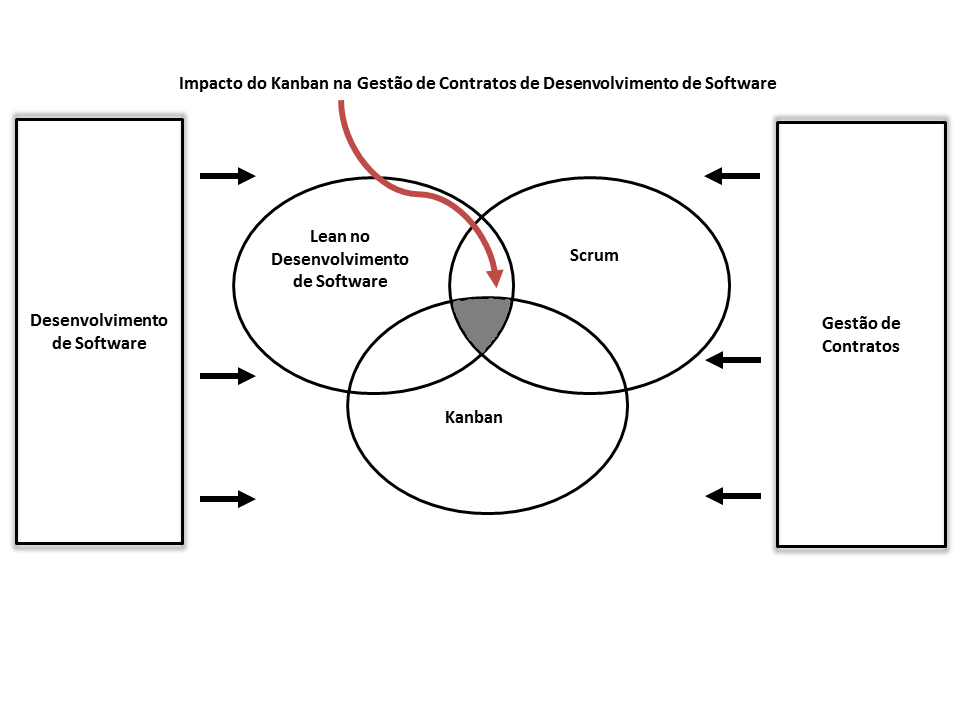
\includegraphics[scale=1.0]{figuras/escopoEC.png}
		
		\caption{Escopo do Estudo de Caso}
		\label{escopo}
		
\end{figure}


Assim, a proposta deste trabalho consiste na investigação, coleta, análise e discussão dos resultados de dados da gestão de contrato de um fornecedor de desenvolvimento de \textit{software} para uma organização pública brasileira. O foco será a análise dos efeitos sobre a entrega de ordens de serviço,  a satisfação do cliente e a qualidade interna do código da solução desenvolvida pela organização, a qual é alinhada com os métodos ágeis, com o pensamento \textit{lean} e com a fase de Gerenciamento do Contrato da Instrução Normativa nº 04.


Para tanto, foi estruturado neste trabalho problema, questões de pesquisa e objetivos conforme ilustrado na Fig. \ref{estrutura}, os quais guiaram o pesquisador durante a fase de coleta de dados.

\begin{figure}[H]
		\centering
		
			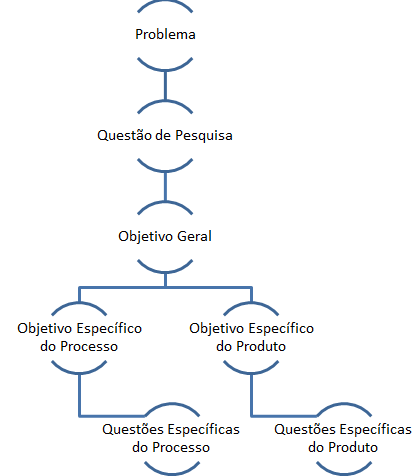
\includegraphics[scale=1.0]{figuras/estruturaEstudo.png}
		\caption{Estrutura do Estudo de Caso}
		\label{estrutura}
	\end{figure}

O problema refere-se ao problema de pesquisa identificado. A questão de pesquisa refere-se a questão de pesquisa que foi derivada do problema. Para responder a questão de pesquisa foram construídos dois GQM's (Goal, Question, Metric) \cite{gqm}. Cada GQM possui um objetivo e questões específicas para coleta de métricas a partir de determinada fonte, a fim de atingir o objetivo e responder a questão de pesquisa do trabalho. Ao todo foram definidas doze questões de pesquisa específicas que serão analisadas no estudo de caso. A definição dessa estrutura está a seguir.

\textbf{Problema:} Alguns contratos de desenvolvimento de \textit{software} da organização não resultaram na entrega do \textit{software} requisitado ao final do contrato.

\textbf{Questão de Pesquisa:} Como o uso de métodos ágeis e do pensamento \textit{lean} na gestão de contratos de fornecedores de desenvolvimento de \textit{software} influenciaram no resultado final do contrato do ponto de vista do gestor de contrato e do fiscal técnico do contrato, que juntos gerenciam o contrato?


\textbf{OE1. Objetivo do Processo:} Analisar a influência do uso de métodos ágeis e do pensamento \textit{lean} na gestão de contrato do contrato do Sistema Integrado de Conhecimento e Gestão (SICG) com a empresa EGL - Engenharia do ponto de vista do gestor de contrato.

\textbf{Questões Específicas do Processo:}


\textbf{QE1.}  Qual a quantidade total de ordens de serviço?

\textbf{Fonte:} Documentação

\textbf{Métrica:} quantidade total de ordens de serviço.
 
\vspace{\onelineskip} 

\textbf{QE2.} Qual a quantidade de ordens de serviço que tiveram entrega de \textit{software} funcional?

\textbf{Fonte:} Documentação

\textbf{Métrica:} quantidade de ordens de serviço de \textit{software}.
 
 \vspace{\onelineskip} 

\textbf{QE3.} Qual a quantidade de ordens de serviço que tiverem entrega apenas de documentação?

\textbf{Fonte:} Documentação

\textbf{Métrica:} quantidade de ordens de serviço de documentação.

 \vspace{\onelineskip} 
 
\textbf{QE4.} Qual a proporção de entrega de \textit{software} funcional?

\textbf{Fonte:} Documentação

\textbf{Métrica:} quantidade de ordens de serviço de \textit{software} que tiveram entrega de \textit{software} funcional /quantidade total de ordens de serviço.

 \vspace{\onelineskip} 

\textbf{QE5.} Qual a duração média de entrega de \textit{software} funcional?

\textbf{Fonte:}Documentação, scrum master, dono do produto, gestor do contrato, fiscal técnico do contrato, coordenador do projeto.

\textbf{Métrica:} duração total das sprints/duração total das sprints que tiveram entrega de \textit{software} funcional.

 \vspace{\onelineskip} 

\textbf{QE6.} Qual a quantidade de ordens de serviço que não teve entrega de \textit{software} funcional e de documentação?

\textbf{Fonte:} Documentação

\textbf{Métrica:} quantidade de ordens de serviço sem entrega de \textit{software} e de documentação.

 \vspace{\onelineskip} 
 
\textbf{QE7.} Qual a porcentagem de requisitos atendidos em cada ordem de serviço?

\textbf{Fonte:} Documentação, dono do produto, gestor do contrato, fiscal técnico do contrato, coordenador do projeto.

\textbf{Métrica:} (requisitos atendidos/requisitos pedidos) * 100.
 
 \vspace{\onelineskip} 

\textbf{QE8.} Quantas multas foram aplicadas no contrato?

\textbf{Fonte:} Documentação, scrum master, dono do produto, gestor do contrato, fiscal técnico do contrato, coordenador do projeto.

\textbf{Métrica}: quantidade de multas.

 \vspace{\onelineskip}  

\textbf{QE9.} Qual o custo de cada sprint e ordem de serviço do projeto?

\textbf{Fonte:} Documentação

\textbf{Métrica}: custo/sprint.

 \vspace{\onelineskip}  

\textbf{QE10.} O quanto de visibilidade do que estava sendo feito o gestor do contrato teve durante o contrato?

\textbf{Fonte:} Dono do produto, gestor do contrato, fiscal técnico do contrato, coordenador do projeto.

\textbf{Métrica:} alto, médio ou baixo. 
 
 \vspace{\onelineskip} 

\textbf{QE11.} Qual o nível de satisfação com o \textit{software} entregue ao final do contrato?

\textbf{Fonte:} Dono do produto, gestor do contrato, fiscal técnico do contrato, coordenador do projeto.

\textbf{Métrica:} muito satisfeito, satisfeito, neutro, insatisfeito, muito insatisfeito.
 
 \vspace{\onelineskip} 

\textbf{OE2. Objetivo do Produto:}Analisar a qualidade do código fonte com o uso de métodos ágeis e do pensamento \textit{lean} na gestão do contrato do contrato do Sistema Integrado 
de Conhecimento e Gestão (SICG) com a empresa EGL - Engenharia do ponto de vista do  e do fiscal técnico do contrato.

\textbf{Questão Específicas do Produto:}

\textbf{QE12.} Qual a qualidade interna do produto entregue até o momento ?

\textbf{Fonte:} Código, scrum master, desenvolvedores, dono do produto, gestor do contrato, fiscal técnico do contrato, coordenador do projeto.

\textbf{Métrica:} bom, excelente, regular e ruim.


\section[Background]{Background}

À luz do levantamento bibliográfico realizado, não foram encontrados estudos que buscassem levantar e analisar os efeitos advindos do uso de metodologias ágeis no contexto da gestão de contratos de fornecedores de desenvolvimento de \textit{software} para organizações públicas brasileiras. O Ácordão nº 2314/2013, relatado no Capítulo 4, traz apenas um levantamento do que foi feito de uso de métodos ágeis pelos órgãos analisados. No entanto, não houve uma coleta e análise de dados, tal qual realizada neste trabalho.

\section[Design]{Design}

Umas das formas de classificar um estudo de caso é com base na identificação de seus propósitos gerais: exploratórios, descritivos, explicativos e avaliativos. Este estudo de caso é classificado como exploratório, pois não esperamos obter uma resposta definitiva para o problema proposto. A ideia é obter uma visão mais acurada do problema para posteriormente realizar uma pesquisa mais aprofundada. Tal escolha foi feita porque o tema escolhido foi pouco explorado até o momento, constituindo apenas a primeira etapa de uma investigação mais ampla e sistemática. 

Uma segunda forma de classificação é relacionada a quantidade de casos: caso único ou casos múltiplos. Considerando as restrições de tempo para realização deste estudo de caso, foi definido o estudo de um caso único (uma organização) e holístico, com uma unidade de análise (um contrato), pois, como mencionado anteriormente, este é um estudo de caso exploratório. Posteriormente, pretende-se ampliar este estudo para múltiplos casos.   

\section[Seleção]{Seleção}

A organização selecionada para este estudo de caso foi o Instituto do Patrimônio Histórico e Cultural (IPHAN). Dentre as organizações analisadas no relatório do Ácordão nº 2314/2013, o IPHAN foi a primeira a adotar o uso de métodos ágeis e pensamento \textit{lean} na gestão de seus contratos. O BACEN, foi o primeiro a buscar a implantação de métodos ágeis. No entanto, foi no contexto de desenvolvimento interno de \textit{software} do órgão. Assim, a seleção justifica-se porque o órgão possuí o primeiro contrato gerenciado com métodos ágeis dentre os contratos das organizações públicas localizadas em Brasília.

\section[Fonte e Método Coleta de Dados]{Fonte e Método de Coleta de Dados}

Os dados foram coletados por meio de entrevistas informais, observações, questionários, análise de documentos dos processos da organização e da base de código fonte de um contrato disponibilizado pelo órgão: o contrato do Sistema Integrado de Conhecimento e Gestão (SICG) com a empresa EGL - Engenharia.

Os questionários tinham o objetivo de coletar dados qualitativos e quantitativos a respeito da organização contratante, do gestor de negócio (cliente) e da empresa contratada no que diz respeito a estrutura organizacional, experiência prévia, satisfação, opiniões, percepções e etc. O dados de observação e entrevistas complementaram os questionários sob o ponto de vista qualitativo.

Os dados quantitativos sobre a execução do processo (solução) foram coletados das 25 ordens de serviço documentadas do projeto. Já os dados da qualidade do código fonte foram coletados de 19 sprints do projeto.

\textbf{Documentos}
\begin{itemize}
\item Processo nº 01450.011592/2010-30, cujo assunto é Contratação de Serviços de Desenvolvimento de \textit{Software} para o Sistema Integrado de Conhecimento e Gestão (SICG). 
\item Processo nº 01450.000845/2012-10, cujo assunto é Gestão de Contrato IPHAN Nº 28/2011 - Desenvolvimento de \textit{Software} para o Sistema Integrado de Conhecimento e Gestão (SICG). 
\item Código Fonte do Sistema Integrado de Conhecimento e Gestão (SICG).
\item Backlog do Produto do Sistema Integrado de Conhecimento e Gestão (SICG).
\end{itemize}

\textbf{Questionários}
\begin{itemize}
\item Questionário para os envolvidos no projeto SICG: tem como objetivo coletar informações dos envolvidos no projeto por parte do IPHAN,  fiscal técnico do contrato, coordenador do projeto e do gestor do contrato, que também representa o papel de dono do produto, e dos envolvidos no projeto por parte da empresa contratada, a EGL - Engenharia, scrum master e desenvolvedores. O contrato aplicada aos envolvidos no projeto pode ser encontrado no Apêndice A.
\end{itemize}

\section[Validade]{Validade}

As principais ameaças aplicáveis aos estudos de caso 
são mencionadas por \citeonline{yin}. Dentre elas, estão a validade do constructo, validade interna, validade externa e confiabilidade.

A validade de constructo diz respeito ao uso de múltiplas fontes de evidência e seleção de informantes chave. Ela ocorre na fase de coleta de dados e está relacionada ao desenvolvimento de um conjunto de métricas para que se saiba exatamente o que medir e quais dados são relevantes para o estudo, de forma a responder as questões de pesquisa. Como apresentado anteriormente, neste trabalho foram utilizadas múltiplas fontes de evidências e os informantes que responderam ao questionário e às entrevistas foram os principais envolvidos no projeto, tanto do órgão contratante quanto da empresa contratada. Além disso, a utilização da técnica GQM direcionou a definição de métricas, procurando-se então a reforçar a validade do constructo.

A validade interna pode ser atingida por meio de diversas estratégias, dentre elas a construção da explanação. Se as conclusões apresentadas pelo estudo de caso correspondem autenticamente a alguma realidade reconhecida pelos próprios envolvidos no projeto, há uma validade interna. Para \citeonline{yin}, o uso de várias fontes de dados e métodos de coleta permite a triangulação, uma técnica para confirmar se os resultados
de diversas fontes e de diversos métodos convergem. Dessa forma é possível aumentar a
validade interna do estudo e aumentar a força das conclusões. Nesta pesquisa houve
triangulação de dados  e de metodologia. A triangulação de dados se deu
pelo uso de base de documentos e código organizacionais, questionários e entrevistas para coletar dados. A triangulação
de métodos ocorreu pelo uso de métodos de coleta quantitativos e qualitativos.

A validade externa diz respeito a estabelecer o quanto as descobertas podem ser generalizadas. Pode-se testar a coerência entre os resultados
do estudo e resultados de outras investigações similares. Para isso, \citeonline{yin} recomenda a replicaçao do estudo em múltiplos casos. Como o escopo deste trabalho é o estudo de um único caso, a validade externa não poderá ser atingida.

E, por fim, a confiabilidade diz respeito a mostrar que se o estudo for repetido utilizando as mesmas fontes de dados, poderá obter-se os mesmos resultados. Para isso, a definição do protocolo do estudo de caso e o 
desenvolvimento de um banco de dados do estudo são táticas para garantir a confiabilidade. Nesse trabalho, o protocolo de estudo de caso é evidenciado nas seções deste capítulo e no questionário, que pode ser encontrado no Apêndice A.


\section[Trabalho de Campo]{Trabalho de Campo}

O trabalho de campo é parte fundamental do estudo de caso. Por meio dele é que os dados para análise serão coletados. Neste trabalho, as entrevistas informais e a triagem dos processos foram realizadas em campo. Os processos disponibilizados pelo orgão eram extensos, mais de 4000 páginas. Por isso, a triagem sobre esses processos foi realizada para solicitação de cópias das partes que mais interessavam para o contexto e objetivos de pesquisa deste estudo.

\section[Análise]{Análise} 

O processo de análise de dados foi composto por três etapas:
\begin{itemize}
\item Redução: refere-se ao processo de seleção, categorização, simplificação e transformação dos dados obtidos, reduzindo-os ao essencial para proporcionar sua análise e interpretação. Os dados qualitativos foram categorizados em: organização, empresa contratada, projeto e solução. Os dados quantitativos foram categorizados de acordo com o tipo de questão específica, e as categorias são: entrega de ordens de serviço, satisfação do cliente e qualidade interna do código fonte.
\item Exibição: consiste na organização dos dados selecionados de forma a possibilitar a análise sistemática das semelhanças e diferenças e seu inter-relacionamento. Os dados foram exibidos, principalmente, por meio de histogramas, tabelas e texto.
\item Conclusão e verificação: consiste em identificar o significado dos dados, suas regularidades, padrões e explicações. A medida que os resultados foram exibidos, uma discurssão e interpretação inicial foi realizada. Posteriormente, na conclusão final foram agrupados os resultados mais relevantes.
\end{itemize}


\section[Considerações Finais do Capítulo]{Considerações Finais do Capítulo}

Este capítulo consistiu em apresentar o projeto de estudo de caso utilizado como base para coleta de dados e análise. No próximo capítulo serão detalhados a organização, a empresa contratada, o objeto do contrato e a solução analisada no estudo de caso e serão apresentados os resultados obtidos para as questões específicas apresentadas neste capítulo assim como a interpretação dos mesmos.